%!TEX program = pdflatex
% SPDX-License-Identifier: MIT
% Copyright (c) 2026 Santhosh Shyamsundar, Santosh Prabhu Shenbagamoorthy — Studio TYTO

%----------------------------------------------------------------------
% Preprint — The Thermodynamic Cost of Knowing
% Public release version
% Compile: cd Docs/Preprint && pdflatex UMST_DoubleSlit_Formal_Verification.tex
%----------------------------------------------------------------------
\documentclass[11pt, a4paper]{article}
\usepackage[T1]{fontenc}
\usepackage[utf8]{inputenc}
\usepackage{mathpazo}
\usepackage[margin=2.5cm, top=2.2cm, bottom=2.2cm]{geometry}
\usepackage{microtype}
\usepackage{amsmath, amssymb, amsthm}
\usepackage{xcolor}
\usepackage{titlesec}
\usepackage{parskip}
\usepackage{enumitem}
\usepackage{booktabs}
\usepackage{needspace}
\usepackage{hyperref}
\usepackage{tikz}
\usetikzlibrary{arrows.meta, positioning}
\usepackage{graphicx}

% --- Monochrome palette (thesis spine) ---
\definecolor{Black}{HTML}{111111}
\definecolor{DimGray}{HTML}{444444}
\definecolor{MidGray}{HTML}{666666}
\definecolor{BorderGray}{HTML}{BBBBBB}
\definecolor{LinkGray}{HTML}{333333}

% --- Figure palette (paper-friendly) ---
\definecolor{FigCyan}{HTML}{2471A3}
\definecolor{FigPurple}{HTML}{6C3483}
\definecolor{FigRed}{HTML}{C0392B}
\definecolor{FigLightBlue}{HTML}{EAF2F8}
\definecolor{FigLightPurple}{HTML}{F4ECF7}

\renewcommand{\familydefault}{\rmdefault}

\titleformat{\section}
    {\fontsize{12}{15}\selectfont\bfseries\color{Black}}
    {\thesection}{0.5em}{}
\titlespacing*{\section}{0pt}{1.0em}{0.4em}

\titleformat{\subsection}
    {\fontsize{11}{14}\selectfont\bfseries\color{DimGray}}
    {\thesubsection}{0.4em}{}
\titlespacing*{\subsection}{0pt}{0.7em}{0.3em}

\hypersetup{
    colorlinks=true,
    linkcolor=Black,
    urlcolor=LinkGray,
    citecolor=DimGray,
    pdftitle={The Thermodynamic Cost of Knowing — Formally Verified},
    pdfauthor={Santhosh Shyamsundar and Santosh Prabhu Shenbagamoorthy, Studio TYTO}
}

\setlength{\parskip}{0.5em}
\setlength{\parindent}{0pt}
\linespread{1.08}
\setlist[enumerate]{leftmargin=1.6em, itemsep=0.3em, topsep=0.2em}
\setlist[itemize]{leftmargin=1.6em, itemsep=0.2em, topsep=0.15em}

% Left-border accent box (thesis spine style)
\newenvironment{leftbox}{%
  \par\vspace{0.5em}%
  \noindent\hspace{0pt}%
  \begin{minipage}[t]{3pt}\color{Black}\rule{3pt}{6.5\baselineskip}\end{minipage}%
  \hspace{10pt}%
  \begin{minipage}[t]{\dimexpr\textwidth-17pt}\small
}{%
  \end{minipage}\par\vspace{0.5em}%
}

\newtheorem{theorem}{Theorem}
\newtheorem{definition}[theorem]{Definition}

% Page numbers (bottom center, small, gray)
\usepackage{fancyhdr}
\pagestyle{fancy}
\fancyhf{}
\renewcommand{\headrulewidth}{0pt}
\fancyfoot[C]{\footnotesize\color{MidGray}\thepage}

\begin{document}

%---------- HEADER ----------
\noindent
{\fontsize{18}{22}\selectfont\bfseries The Thermodynamic Cost of Knowing}

\vspace{0.3em}
\noindent{\fontsize{13}{16}\selectfont\color{DimGray}\itshape Observation as Irreversible Payment --- A Formally Verified Bridge from Quantum Measurement to Classical Thermodynamics}

\vspace{0.4em}
\noindent{\fontsize{10}{13}\selectfont\color{MidGray}%
$V^2 \;+\; \bigl(1 - H_{\mathrm{bits}}(\rho)\bigr) \;\le\; 1
\qquad\Longrightarrow\qquad
Q \;\ge\; k_B T \ln 2 \;\cdot\; \bigl(1 - V^2\bigr)$\\[3pt]
\textit{Every fraction of a bit of which-path information causes a proportional destruction of interference---and each fraction carries an exact Landauer cost.}}

\vspace{0.5em}
\noindent{\small\color{MidGray}\textsf{TECHNICAL NOTE}\quad\rule[0.35ex]{2em}{0.5pt}\quad March 2026}

\vspace{0.3em}
{\small\color{MidGray}%
\textbf{Santhosh Shyamsundar} --- Studio TYTO; IAAC Barcelona\quad\texttt{santhoshshyamsundar@tyto.studio}\\[2pt]
\textbf{Santosh Prabhu Shenbagamoorthy} --- Studio TYTO; IAAC Barcelona\quad\texttt{santosh@tyto.studio}\\[3pt]
\textit{Lean\,4 + Mathlib, Haskell QuickCheck, Coq/Rocq, Agda, Python}}

\vspace{0.5em}
{\color{Black}\rule{\textwidth}{2.5pt}}

%---------- TEASER IMAGE ----------
\begin{figure}[htbp]
\centering
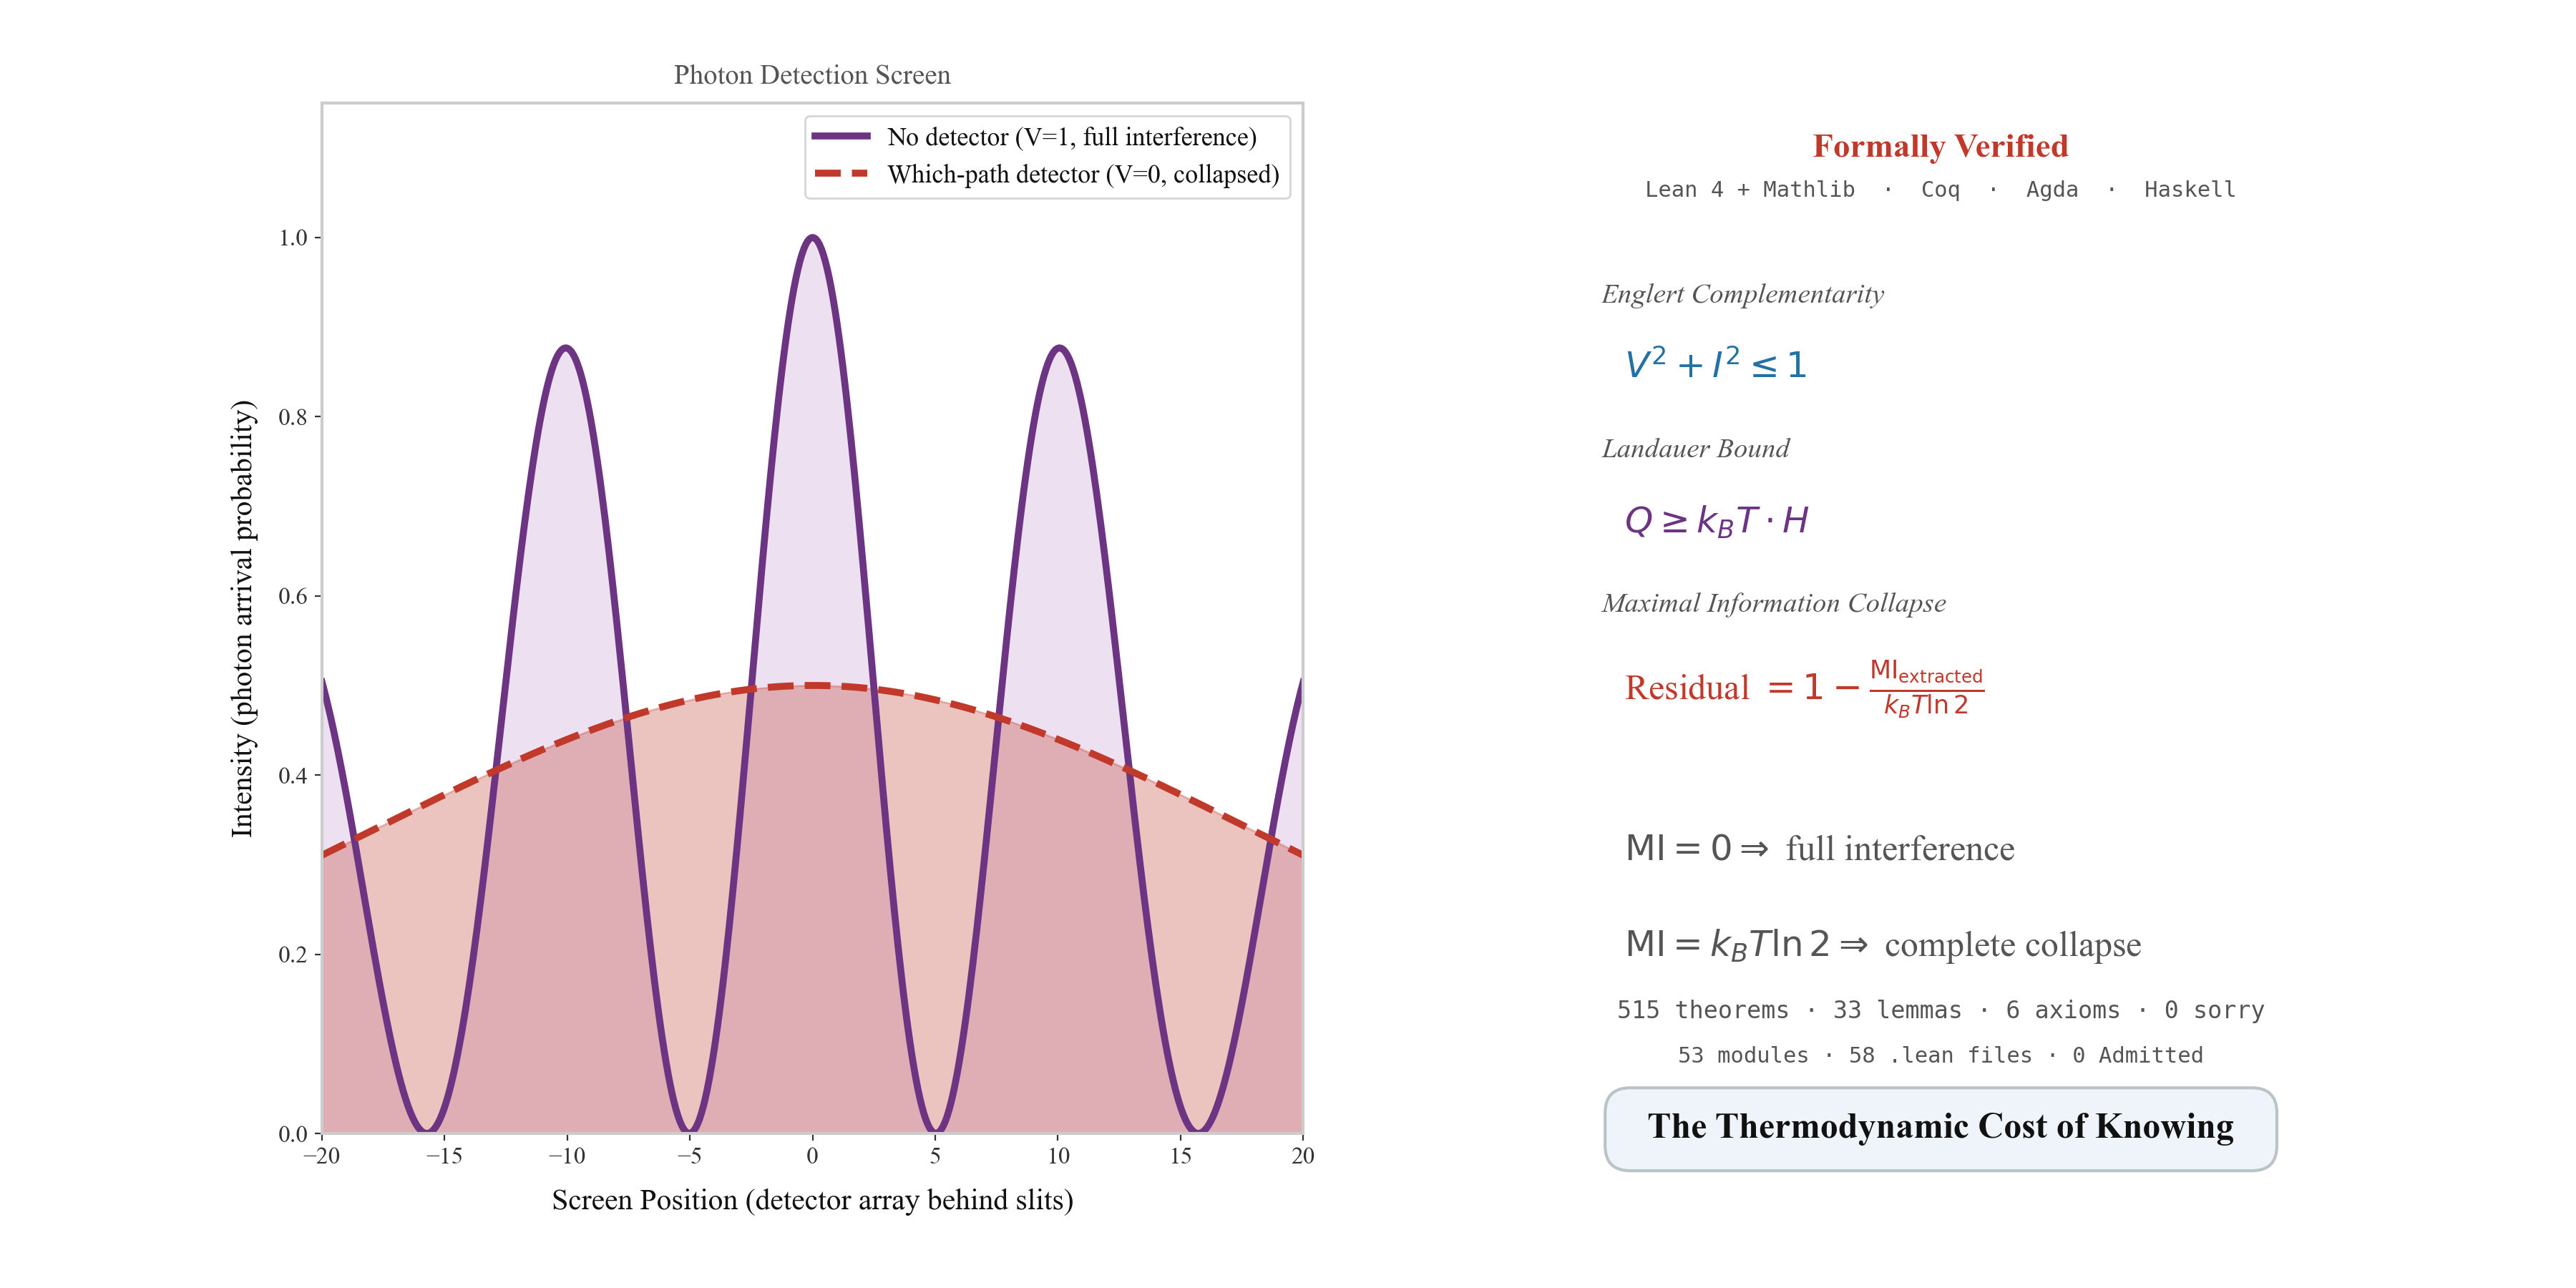
\includegraphics[width=1.0\textwidth]{../Media/teaser-paper.png}
\caption{\textbf{Visual summary of the formalization out-of-the-box.} The extracted which-path information acts as an irreversible measurement channel, systematically degrading fringe visibility. The exact thermodynamic cost is bounded by Landauer's principle, forming a strict tradeoff between coherence and dissipation rigorously quantified in Lean 4.}
\vspace{-1em}
\label{fig:teaser}
\end{figure}

%---------- CORE RESULT ----------

\begin{leftbox}
\textbf{Core Result: Principle of Maximal Information Collapse.}
When an observer extracts which-path information from a quantum system, the residual coherence capacity is:
\[
\text{Residual Coherence} = 1 - \frac{\text{MI}_{\text{extracted}}}{k_B T \ln 2} \;\in\; [0,\,1]
\]
Extract 0 bits $\implies$ full interference.\quad Extract 1 bit $\implies$ complete decoherence.\\[3pt]
\textbf{Crucially, observation is not binary.} Partial measurement extracts a \emph{fraction} of a bit, causing proportional decoherence along the Englert curve $V = \sqrt{1 - I^2}$.\\[3pt]
\textit{Machine-checked in Lean\,4 with Mathlib.\; \textbf{515 theorems, 0 \texttt{sorry}, 6 explicit axioms} (corresponding to physical principles or pending Mathlib infrastructure).}
\end{leftbox}

%---------- MOTIVATION ----------
\section{Motivation and Prior Work}

The double-slit experiment is the canonical demonstration of quantum mechanics~\cite{feynman1965, vonneumann1932}: a single particle interferes with itself, producing fringes on a detection screen---unless an observer determines \emph{which slit} the particle traversed, in which case the fringes vanish~\cite{bohr1928}. This complementarity between path information and interference visibility was first quantified by Wootters and Zurek~\cite{wootters1979} and Greenberger and Yasin~\cite{greenberger1988}, then sharpened to Englert's tight inequality $V^2 + I^2 \le 1$~\cite{englert1996}.

Though well established, this tradeoff is typically treated as a purely quantum phenomenon, disconnected from classical thermodynamics. The decoherence programme~\cite{zurek2003, schlosshauer2005} explains the \emph{mechanism} of the quantum-to-classical transition but does not quantify its \emph{thermodynamic cost}. This gap leaves a fundamental question open: what is the minimum energy required, in joules, to destroy a given fraction of interference?

Our prior work on the \textbf{Unified Material-State Tensor (UMST)} framework~\cite{umst-formal, fcpI, fcpII} established a formally verified thermodynamic gate for continuum materials: a Kleisli-categorical structure enforcing conservation laws (mass, energy, hydration bounds) with graded admissibility. The key insight was that \emph{admissibility is compositional but not transitive}---two individually valid transitions can compose to an inadmissible one, proved via triangle-inequality grading (the \texttt{admissibleTrans} counterexample: densities $\{0, 99, 198\}$ kg/m$^3$ with $\delta = 100$).

The present work extends this framework to quantum measurement. We show that the act of measurement is not a mysterious ``collapse'' but a \emph{thermodynamic transaction}: extracting which-path information requires physical work bounded below by Landauer's principle~\cite{landauer1961, bennett1982} ($Q \ge k_B T \ln 2$ per bit, experimentally confirmed~\cite{berut2012}), and this energy expenditure is \emph{mathematically identical} to the destruction of quantum coherence.

%---------- MATHEMATICAL FOUNDATIONS ----------
\section{Mathematical Foundations}

\subsection{The Quantum State (Path Qubit)}

The formalization models the spatial degree of freedom of a particle traversing a double-slit interferometer as a two-level quantum system (a qubit). The state is represented by a \textbf{density matrix} $\rho \in \mathbb{C}^{2 \times 2}$ satisfying three constraints:

\begin{enumerate}
\item \textbf{Hermitian:} $\rho = \rho^\dagger$ (the matrix equals its conjugate transpose).
\item \textbf{Positive semi-definite (PSD):} For any state vector $|\psi\rangle$, $\langle \psi | \rho | \psi \rangle \ge 0$.
\item \textbf{Unit trace:} $\mathrm{Tr}(\rho) = \rho_{00} + \rho_{11} = 1$.
\end{enumerate}

The diagonal elements are the classical Born weights---probabilities of traversing each slit:
\[
p_0 = \rho_{00}, \qquad p_1 = \rho_{11}, \qquad p_0, p_1 \ge 0, \qquad p_0 + p_1 = 1
\]
The off-diagonal element $\rho_{01} = \rho_{10}^*$ is the complex \textbf{coherence}: the quantum interference capability. Its magnitude $|\rho_{01}|$ directly controls fringe contrast; its phase determines the spatial alignment of the interference pattern.

\subsection{Path Distinguishability and Fringe Visibility}

Two physical observables characterize the double-slit complementarity:

\begin{definition}[Path Distinguishability]
$I = |p_0 - p_1| \in [0, 1]$. When $p_0 = p_1 = \tfrac{1}{2}$, the observer has zero which-path knowledge ($I = 0$); when $p_0 = 1$ and $p_1 = 0$, the path is fully determined ($I = 1$).
\end{definition}

\begin{definition}[Fringe Visibility]
$V = 2|\rho_{01}| \in [0, 1]$. This is proportional to the magnitude of quantum coherence. $V = 1$ corresponds to maximal interference fringes; $V = 0$ means no interference pattern at all.
\end{definition}

\subsection{Englert's Complementarity Relation}

The inequality $V^2 + I^2 \le 1$ is not a postulate---it is a \emph{theorem} derivable from the PSD constraint alone. Because $\rho$ is positive semi-definite, its determinant is non-negative:
\[
\det(\rho) = \rho_{00}\rho_{11} - |\rho_{01}|^2 \ge 0 \qquad\implies\qquad |\rho_{01}|^2 \le p_0 p_1
\]
Substituting into the definitions of $V$ and $I$:
\[
V^2 + I^2 = 4|\rho_{01}|^2 + (p_0 - p_1)^2 \le 4p_0 p_1 + (p_0 - p_1)^2 = (p_0 + p_1)^2 = 1
\]
This corresponds to the Lean theorem \texttt{complementarity\_fringe\_path}
(\texttt{QuantumClassicalBridge}). Any gain in which-path distinguishability
$I$ mathematically necessitates a rigid destruction of interference visibility $V$.

%---------- MEASUREMENT CHANNEL ----------
\section{The Measurement Channel}

The act of a detector at the slits is modeled as a \textbf{Kraus trace-preserving completely positive map}. An ideal which-path interaction is the L\"uders dephasing channel:
\[
\mathcal{E}_{\mathrm{path}}(\rho) = \Pi_0 \rho \Pi_0 + \Pi_1 \rho \Pi_1
\]
where $\Pi_0 = |0\rangle\langle 0|$ and $\Pi_1 = |1\rangle\langle 1|$ are the spatial projectors onto each slit. These satisfy the Kraus properties proved in the repository (\texttt{MeasurementChannel.lean}):

\begin{itemize}
\item \textbf{Self-adjoint:} $\Pi_i = \Pi_i^\dagger$
\item \textbf{Idempotent:} $\Pi_i^2 = \Pi_i$
\item \textbf{Orthogonal:} $\Pi_0 \Pi_1 = 0$
\item \textbf{Complete:} $\Pi_0 + \Pi_1 = \mathbb{I}$ (trace-preserving)
\end{itemize}

This channel preserves the diagonal entries ($p_0$ and $p_1$ are unchanged) but strictly forces the off-diagonal coherences to zero ($\rho_{01} \to 0$), which forces $V \to 0$ post-measurement. This is the formal content of wavefunction collapse on the path basis: not a mysterious event, but a mathematically precise trace-preserving operation whose thermodynamic cost we quantify next.

%---------- PROOF ARCHITECTURE ----------
\section{Proof Architecture}

The formalization is structured as a \emph{closed chain} from quantum states through measurement to thermodynamic cost.

\begin{figure}[htbp]
\centering
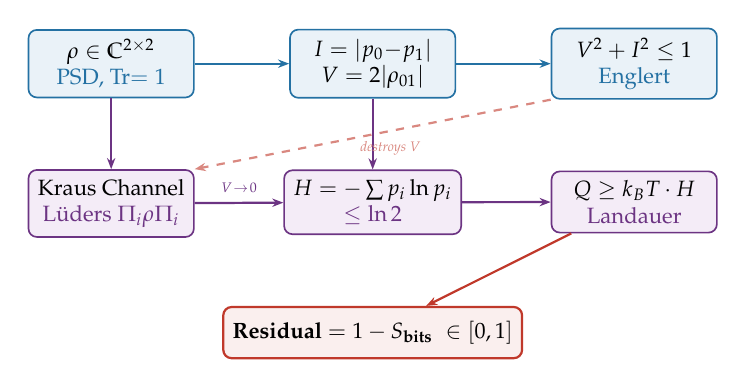
\begin{tikzpicture}[
  qbox/.style={draw=FigCyan, fill=FigLightBlue, rounded corners=3pt, minimum width=2.1cm, minimum height=0.65cm, align=center, font=\footnotesize, line width=0.6pt},
  ibox/.style={draw=FigPurple, fill=FigLightPurple, rounded corners=3pt, minimum width=2.1cm, minimum height=0.65cm, align=center, font=\footnotesize, line width=0.6pt},
  rbox/.style={draw=FigRed, fill=FigRed!8, rounded corners=3pt, minimum width=3.4cm, minimum height=0.65cm, align=center, font=\footnotesize\bfseries, line width=0.8pt},
  qarrow/.style={-{Stealth[length=4pt]}, thick, color=FigCyan},
  iarrow/.style={-{Stealth[length=4pt]}, thick, color=FigPurple},
  rarrow/.style={-{Stealth[length=4pt]}, thick, color=FigRed}
]
\node[qbox] (rho) {$\rho \in \mathbb{C}^{2\times 2}$\\\color{FigCyan}PSD, Tr$=1$};
\node[qbox, right=1.2cm of rho] (iv) {$I = |p_0{-}p_1|$\\$V = 2|\rho_{01}|$};
\node[qbox, right=1.2cm of iv] (comp) {$V^2 + I^2 \le 1$\\\color{FigCyan}Englert};
\node[ibox, below=0.9cm of rho] (kraus) {Kraus Channel\\\color{FigPurple}L\"uders $\Pi_i \rho \Pi_i$};
\node[ibox, below=0.9cm of iv] (ent) {$H = -\sum p_i \ln p_i$\\\color{FigPurple}$\le \ln 2$};
\node[ibox, below=0.9cm of comp] (land) {$Q \ge k_B T \cdot H$\\\color{FigPurple}Landauer};
\node[rbox, below=0.9cm of ent] (pmic) {Residual $= 1 - S_{\text{bits}}$\;\;$\in [0,1]$};

\draw[qarrow] (rho) -- (iv);
\draw[qarrow] (iv) -- (comp);
\draw[iarrow] (rho) -- (kraus);
\draw[iarrow] (kraus) -- node[above, font=\tiny\color{FigPurple}]{$V\!\to\!0$} (ent);
\draw[iarrow] (iv) -- (ent);
\draw[iarrow] (ent) -- (land);
\draw[rarrow] (land) -- (pmic);
\draw[-{Stealth[length=4pt]}, dashed, thick, color=FigRed!60] (comp.south west) -- node[below, font=\tiny\itshape, color=FigRed!60, pos=0.45]{destroys $V$} (kraus.north east);
\end{tikzpicture}
\caption{\textbf{Proof Architecture Pipeline.} \textbf{Top row (cyan):} The quantum state $\rho$ yields observables $I$ and $V$, bounded by Englert complementarity. \textbf{Middle row (purple):} The L\"uders channel extracts which-path information, producing diagonal entropy $H$ and incurring a Landauer cost. \textbf{Bottom (red):} The Principle of Maximal Information Collapse unifies these into a single residual-coherence metric.}
\label{fig:architecture}
\end{figure}

%---------- PMIC ----------
\section{The Principle of Maximal Information Collapse}

\subsection{Diagonal Information Entropy}

The diagonal von Neumann entropy quantifies the classical uncertainty in the Born weights:
\[
H = -p_0 \ln p_0 - p_1 \ln p_1 \qquad (\le \ln 2 \text{ nats})
\]
This is the Shannon entropy of the computational-basis probabilities, capped at $\ln 2$ for a binary system. We normalize this to bit-equivalents:
\[
S_{\text{bits}} = \frac{H}{\ln 2} \;\in\; [0, 1]
\]

\subsection{The Landauer Cost}

Extracting the which-path bit from the quantum system to a macroscopic register incurs a strict physical lower bound on heat dissipation via Landauer's Principle~\cite{landauer1961}:
\[
Q \;\ge\; k_B T \ln 2 \;\cdot\; S_{\text{bits}}
\]
This cost is bounded above by a single Landauer bit-energy $k_B T \ln 2$, because the path qubit carries at most one bit of information. The bound has been experimentally confirmed to within statistical error~\cite{berut2012}.

\subsection{Residual Coherence Capacity}

The \textbf{residual coherence capacity} after information extraction is formally proved to satisfy:
\[
\text{Residual} = 1 - S_{\text{bits}} \;\in\; [0,\,1]
\]
with tight bounds at both endpoints:
\begin{itemize}
\item $S_{\text{bits}} = 0$ (no information extracted) $\implies$ Residual $= 1$ (full visibility possible).
\item $S_{\text{bits}} = 1$ (maximum 1-bit extraction) $\implies$ Residual $= 0$ (complete decoherence).
\end{itemize}

We also prove the \textbf{cost--coherence identity}:
\[
Q = k_B T \ln 2 \cdot (1 - \text{Residual})
\]
The thermodynamic cost is \emph{exactly proportional} to the fraction of coherence destroyed. A concrete \texttt{ErasureProcess} structure in Lean enforces $\text{dissipatedHeat} \ge \text{landauerCostDiagonal}$ via the Second Law.

\subsection{The Continuous Tradeoff}

The standard textbook narrative presents measurement as all-or-nothing: ``observe and the fringes vanish.'' The Englert relation reveals a \emph{continuum}: a probe that extracts $I = 0.3$ bits of which-path information reduces fringe visibility to $V = \sqrt{1 - 0.09} \approx 0.95$---the interference pattern is barely disturbed. At $I = 0.7$ the fringes are heavily suppressed ($V \approx 0.71$). Full decoherence requires extracting the \emph{entire} bit. Every point on the curve $V^2 + I^2 = 1$ is physically realizable, and each carries a proportional Landauer cost. This continuous tradeoff is precisely what the residual-capacity framework captures and what the Lean formalization proves.

This closes the self-consistent loop: the macroscopic energy expenditure of the intelligent probe maps \emph{directly} to the microscopic destruction of interference.

%---------- THEOREM TABLE ----------
\needspace{10\baselineskip}
\section{What Is Formally Proved}

Every row below is a machine-checked theorem in Lean\,4 with Mathlib~\cite{lean4, mathlib2020}---no \texttt{sorry} in these modules. The repository contains one Phase-5 placeholder: general unital DPI / Klein in \texttt{DataProcessingInequality.lean} (see \texttt{Lean/VERIFY.md}).

\vspace{0.3em}
{\small
\begin{tabular}{@{}lll@{}}
\toprule
\textbf{Theorem} & \textbf{Statement} & \textbf{Module} \\
\midrule
Englert complementarity & $V^2 + I^2 \le 1$ & \texttt{QuantumClassicalBridge} \\
Which-path collapse & $V \to 0$ after L\"uders channel & \texttt{MeasurementChannel} \\
Projector properties & self-adjoint, idempotent, orthogonal, TP & \texttt{MeasurementChannel} \\
Density matrix diagonals & PSD $\implies$ $p_i \ge 0$, $\sum p_i = 1$, $p_i \le 1$ & \texttt{DensityState} \\
Diagonal entropy bound & $H_{\text{diag}} \le \ln 2$ & \texttt{InfoEntropy} \\
Landauer cost cap & cost $\le k_B T \ln 2$ & \texttt{LandauerBound} \\
Path entropy $\le 1$ bit & $S_{\text{bits}} \in [0, 1]$ & \texttt{LandauerBound} \\
Maximal collapse & $S_{\text{bits}} = 1 \implies \text{Residual} = 0$ & \texttt{LandauerBound} \\
Null preservation & $S_{\text{bits}} = 0 \implies \text{Residual} = 1$ & \texttt{LandauerBound} \\
Cost--coherence identity & $Q = k_B T \ln 2 \cdot (1 - \text{Residual})$ & \texttt{LandauerBound} \\
Erasure $\ge$ bound & dissipatedHeat $\ge$ landauerCostDiagonal & \texttt{LandauerBound} \\
Which-path invariance & Landauer cost unchanged by measurement & \texttt{LandauerBound} \\
Gate enforcement & admissibility + Landauer + cap in one & \texttt{DoubleSlit} \\
\bottomrule
\end{tabular}}

%---------- ASSUMPTIONS AND SCOPE ----------
\section{Assumptions and Scope}

The formalization makes the following explicit assumptions---none of which are proof gaps in the stated formal theorems. They are \emph{scope control}: boundaries on what the current verification covers.

\begin{enumerate}
\item \textbf{Standard finite-dimensional QM} as encoded in Mathlib: complex matrices, \texttt{PosSemidef}, trace, Kraus form for CPTP maps.
\item \textbf{Path qubit only:} Hilbert space $\texttt{Fin 2} \to \mathbb{C}$ for the which-path degree of freedom. No spatial fringe pattern in position/momentum bases within this formal layer.
\item \textbf{Coarse readout $(I, V)$:} Defined proxies, not derived von Neumann entropy of an apparatus.
\item \textbf{Diagonal entropy:} \texttt{vonNeumannDiagonal} uses computational-basis diagonals; for general pure states with coherence, this can differ from the full $S(\rho) = -\mathrm{Tr}(\rho \log \rho)$.
\item \textbf{Landauer layer:} The term \texttt{landauerCost\-Diagonal} is a scale $k_B T \ln 2 \times H_{\mathrm{bits}}$---not a claim that measured heat equals this without an explicit erasure/bath model.
\end{enumerate}

\noindent\textbf{What is not claimed:}
\begin{itemize}
\item Derivation from a relativistic or gravitational UMST layer.
\item Identification of $I$ with a specific experimental which-path meter without calibration axioms.
\item Full unital quantum DPI / Klein inequality on compound systems:
stated as \texttt{axiom} (pending Mathlib matrix-log); qubit-tier DPI and
quantum mutual information $I(A\!:\!B)=S(A)+S(B)-S(AB)$ are fully proved.
\item Mixed ensembles as formal convex sums in \texttt{DensityState} (future).
\item Certified ODE/PPO solver convergence/stability claims without a dedicated numerical analysis layer.
\end{itemize}

%---------- CONNECTION ----------
\section{Connection to the UMST Framework}

This work extends the UMST formal verification stack in three directions:

\begin{enumerate}
\item \textbf{From classical to quantum admissibility.} The original UMST gate checks mass conservation, Clausius-Duhem entropy, and hydration bounds on \emph{classical} states (over $\mathbb{Q}$ with \texttt{AdmissibleN}). Here, the gate operates on \emph{quantum} density matrices: the projector $\Pi_i \rho \Pi_i$ is the measurement-channel analogue, and admissibility is enforced by Englert complementarity plus the Landauer bound.

\item \textbf{From material hydration to information erasure.} In the original framework, the Helmholtz free energy $\psi(\alpha)$ governs the cost of hydration transitions. Here, the diagonal von Neumann entropy $H(\rho)$ governs the cost of information extraction. Both are monotone hooks: increasing hydration lowers free energy; increasing path information lowers residual coherence. The Galois adjunction \texttt{EpistemicGalois} makes this connection explicit.

\item \textbf{From counterexample to principle.} The discovery that \texttt{admissibleTrans} is \emph{refutable} led to graded admissibility. The analogous quantum insight is that partial measurements compose non-trivially: two weak measurements each extracting $< 1$ bit can together extract the full bit, collapsing coherence entirely. The residual-capacity framework captures this compositional structure.
\end{enumerate}

%---------- VERIFICATION ----------
\section{Verification Stack}

\vspace{0.2em}
{\small
\begin{tabular}{@{}llll@{}}
\toprule
\textbf{Layer} & \textbf{Tool} & \textbf{Scope} & \textbf{Status} \\
\midrule
Formal proof & Lean 4 + Mathlib & 53 mod., 515 thm., 33 lem. & \textbf{0 sorry}, \textbf{6 axioms} \\
Property testing & Haskell QuickCheck & 14 properties + sanity & \textbf{All pass} \\
Numerical sim & Python (stdlib + QuTiP) & 87 unit tests, 4 sims & \textbf{All pass} \\
Cross-language & Coq + Agda & 9 Coq + 11 Agda mod. & \textbf{0 Admitted}; Agda \textbf{clean} \\
\bottomrule
\end{tabular}}

\vspace{0.3em}
\noindent The Python simulator demonstrates the collapse visually: as which-path information $I$ increases from 0 to 1, the interference pattern progressively flattens, tracking the $V = \sqrt{1 - I^2}$ Englert curve exactly. The accompanying animated GIF (\texttt{Docs/Media/double-slit-collapse.gif}) visualizes this continuous tradeoff across 60 frames.

\vspace{0.5em}
{\color{Black}\rule{\textwidth}{1pt}}
\vspace{0.2em}

\noindent{\small\textit{Repository:} \texttt{github.com/tytolabs/umst-formal-double-slit} \quad\textbar\quad \textit{DOI:} \href{https://doi.org/10.5281/zenodo.19159660}{10.5281/zenodo.19159660} \quad\textbar\quad \textit{License:} MIT \quad\textbar\quad \textit{Build:} \texttt{cd Lean \&\& lake build}}

\noindent{\footnotesize\color{MidGray}\copyright\;2026 Studio TYTO $\cdot$ \texttt{github.com/tytolabs}}

\vspace{1em}
\needspace{14\baselineskip}
\noindent{\footnotesize\color{MidGray}\textbf{Acknowledgments.} Portions of this work were developed in collaboration with advanced large-language-model tools. Claude Opus and Sonnet 4.6 (Anthropic) provided surgical precision during drafting and refinement. Gemini 3.1 Pro High (Google) offered exceptional large-context planning and file management. Grok 4.20 by xAI and its collaborative reasoning team contributed core mathematical and scientific reasoning. The Cursor code editor, Composer, Claude Code, and Antigravity supported seamless implementation and agentic file management.

\textit{Critical Disclaimer:} The large-language models assisted with exploration, drafting, and code scaffolding---never with the validity of formal proofs. All theorems were machine-checked by their respective compilers (Lean\,4, Coq/Rocq, Agda), which accept only well-typed terms, never persuasive arguments.

The mathematical reality captured in this repository rests entirely on the foundational work of the open-source community. We acknowledge the maintainers and contributors of the Lean\,4 theorem prover and Mathlib, the Coq/Rocq proof assistant, and the Agda dependently typed language and standard library. The simulation and property-checking layers depend on the rigor of Haskell (GHC, Cabal, QuickCheck) and Python 3 (NumPy, SciPy, Matplotlib). Without the decades of collective effort embedded in these compilers and libraries, formally verified physics of this nature would not be possible.}
\vspace{1em}

%---------- REFERENCES ----------
\begingroup
\footnotesize
\begin{thebibliography}{99}

%--- Our work ---
\bibitem{umst-formal} S.~Shyamsundar and S.\,P.~Shenbagamoorthy, ``Formal Verification and Categorical Semantics for the UMST/DUMSTO Thermodynamic Gate,'' \texttt{umst-formal} (double-slit extension track), GitHub, 2026. Lean\,4: 515 \texttt{theorem}s, 53 \texttt{lakefile} roots, 58 \texttt{.lean} files; 0 \texttt{sorry}; 6 \texttt{axiom}s (see \texttt{PROOF-STATUS.md}).

\bibitem{fcpI} S.~Shyamsundar and S.\,P.~Shenbagamoorthy, ``Towards Unified Material-State Tensors for Physics-Gated AI: Thermodynamic Admissibility as Constitutional Constraint,'' Zenodo, 2026. \texttt{doi:10.5281/zenodo.18768547}

\bibitem{fcpII} S.\,P.~Shenbagamoorthy and S.~Shyamsundar, ``Epistemic Sensing Architecture for Physics-Constrained Material Characterization,'' Zenodo, 2026. \texttt{doi:10.5281/zenodo.18894710}

%--- Quantum foundations ---
\bibitem{bohr1928} N.~Bohr, ``The quantum postulate and the recent development of atomic theory,'' \textit{Nature}, 121:580--590, 1928.

\bibitem{feynman1965} R.\,P.~Feynman, R.\,B.~Leighton, and M.~Sands, \textit{The Feynman Lectures on Physics}, Vol.\,III, Ch.\,1, Addison-Wesley, 1965.

\bibitem{vonneumann1932} J.~von~Neumann, \textit{Mathematische Grundlagen der Quantenmechanik}, Springer, 1932.

\bibitem{wootters1979} W.\,K.~Wootters and W.\,H.~Zurek, ``Complementarity in the double-slit experiment,'' \textit{Phys.\ Rev.\ D}, 19(2):473--484, 1979.

\bibitem{greenberger1988} D.\,M.~Greenberger and A.~Yasin, ``Simultaneous wave and particle knowledge in a neutron interferometer,'' \textit{Phys.\ Lett.\ A}, 128:391--394, 1988.

\bibitem{englert1996} B.-G.~Englert, ``Fringe visibility and which-way information: An inequality,'' \textit{Phys.\ Rev.\ Lett.}, 77(11):2154--2157, 1996.

%--- Thermodynamics of information ---
\bibitem{landauer1961} R.~Landauer, ``Irreversibility and heat generation in the computing process,'' \textit{IBM J.\ Res.\ Dev.}, 5(3):183--191, 1961.

\bibitem{bennett1982} C.\,H.~Bennett, ``The thermodynamics of computation---a review,'' \textit{Int.\ J.\ Theor.\ Phys.}, 21:905--940, 1982.

\bibitem{berut2012} A.~B\'{e}rut \textit{et al.}, ``Experimental verification of Landauer's principle linking information and thermodynamics,'' \textit{Nature}, 483:187--189, 2012.

%--- Decoherence ---
\bibitem{zurek2003} W.\,H.~Zurek, ``Decoherence, einselection, and the quantum origins of the classical,'' \textit{Rev.\ Mod.\ Phys.}, 75:715--775, 2003.

\bibitem{schlosshauer2005} M.~Schlosshauer, ``Decoherence, the measurement problem, and interpretations of quantum mechanics,'' \textit{Rev.\ Mod.\ Phys.}, 76:1267--1305, 2005.

\bibitem{nielsen2000} M.\,A.~Nielsen and I.\,L.~Chuang, \textit{Quantum Computation and Quantum Information}, Cambridge Univ.\ Press, 2000.

%--- Formal verification ---
\bibitem{lean4} L.~de~Moura and S.~Ullrich, ``The Lean~4 Theorem Prover and Programming Language,'' \textit{CADE-28}, pp.\,625--635, Springer, 2021.

\bibitem{mathlib2020} The Mathlib Community, ``The Lean Mathematical Library,'' \textit{CPP 2020}, pp.\,367--381, ACM, 2020.

\bibitem{avigad2017} J.~Avigad, J.~H\"{o}lzl, and L.~Serafin, ``A formally verified proof of the central limit theorem,'' \textit{J.\ Automated Reasoning}, 59:389--423, 2017.

\end{thebibliography}
\endgroup

\end{document}
